\section{Description of HF Calorimeters}

The Hadron Forward (HF) calorimeters in the Compact Muon Solenoid (CMS)
experiment at the Large Hadron Collider (LHC) cover a large pseudorapidity
range, $3 \le |\eta| \le 5$, and thus significantly improve jet detection and the missing transverse energy resolution which are essential in top quark production studies, Standard Model Higgs, and all SUSY particle searches~\cite{CMSTP:1994,CMSTP:1997}.

The CMS has two hadronic forward calorimeters, HF- and HF+, each essentially a cylindrical steel structure with an inner radius of 12.5 cm to accommodate the beam pipe, an outer radius of 130.0 cm, and with the front face located 11.15 m from the interaction point. Both calorimeters are wrapped by hermetic radiation shielding of 40 cm thick steel, 40 cm of concrete, and 5 cm of polyethylene, with a large steel plug in the back of each detector.

\begin{figure}[!h]
   \begin{center}
      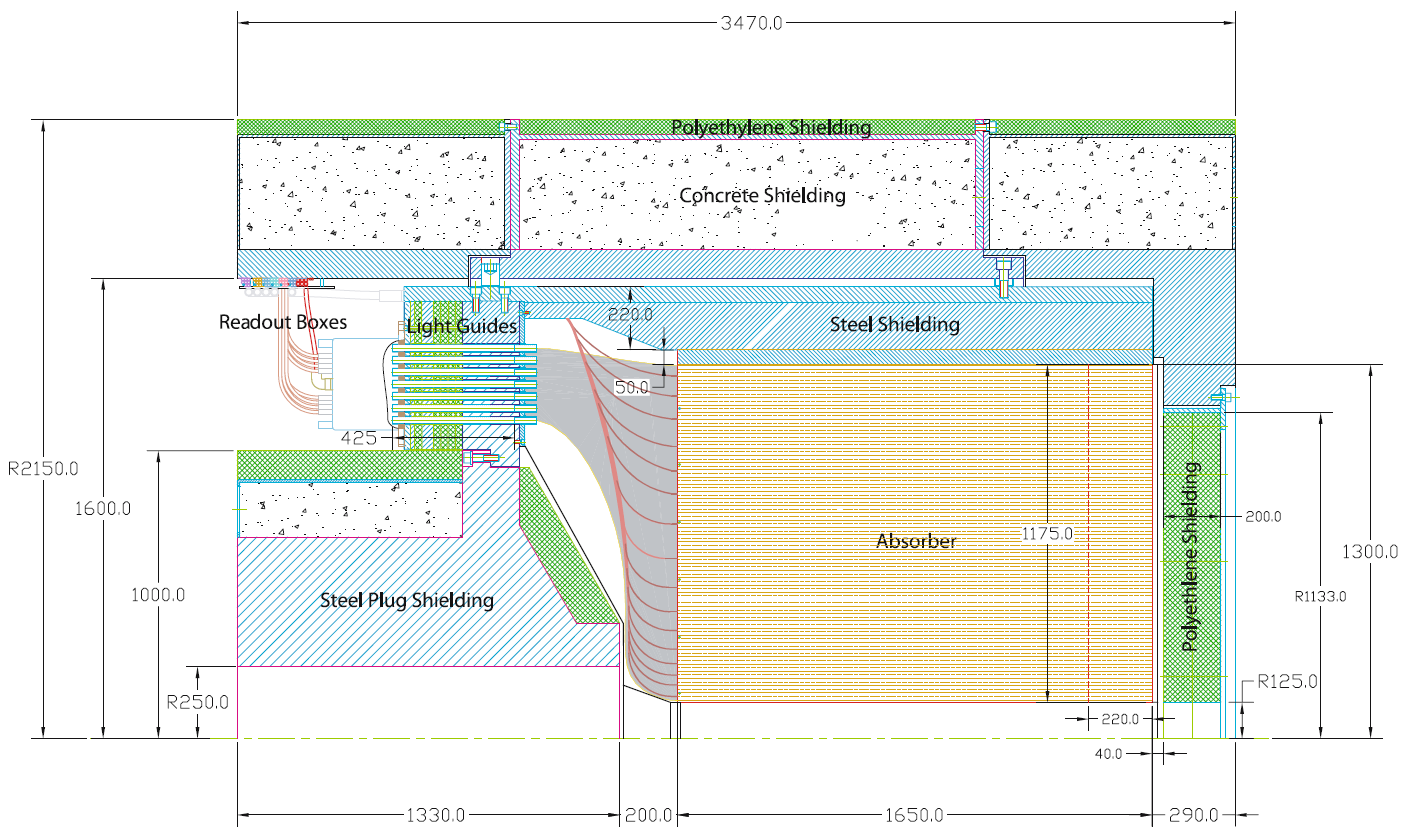
\includegraphics[width=1.\textwidth]{figures/ch_hfcalibration/HF_Calorimeter.png}
      \caption{Cross section of the HF calorimeter. IP is to the right}
      \label{fig:hf_description_crosssectionview}
   \end{center}
\end{figure}

Figure~\ref{fig:hf_description_crosssectionview} displays a cross sectional view of an HF calorimeter. Each HF side is azimuthally subdivided into 18 20 de wedges composed of 5 mm thick grooved steel plates that perform as absorbers. The plate grooves run parallel to the beam line and are spaced 5.0 $\pm$ 0.1 mm center-to-center, each housing a single optical fiber. Each fiber consists of a fused-silica, also referred to as quartz, core of 600 $\pm$ 10 mum diameter, layered to an outer diameter of 630 $^{+5}_{-10}$ mum with polymer hard-clad, and surrounded to a final diameter of 800 $\pm$ 30 mum with protective acrylate buffer. The optical attenuation for each fiber scales as $a(\lambda)(D/D_0)^{b(\lambda)}$, where $a$ and $b$ characterize radiation hardness, $D$ is the accumulated dose, and $D_0$ is a reference dose (100 MRad)~\cite{HFCC:2008}. Each
wedge's fibers are bundled to form 24 towers, each with 0.175 x 0.175 ($\Delta\eta$ x $\Delta\phi$) angular span, with exception in angular span for the 2 towers formed closest to the beam pipe. The bundled fibers are held in ferrules that illuminate one end of air-core light guides penetrating shielding of steel, lead, and polyethylene necessary for the readout boxes. The air-core light
guides are hollow tubes inlined with highly reflective metal-coated sheets and are coupled to standard bialkaline, 8-stage R7525 Hamamatsu photomultiplier tubes (PMT) with a borosilicate glass window. During LS1 R7525 PMTs (Old) were replaced by metal case Hamamatsu R7600 PMTs (New), which have a thinner front window.

Cherenkov light forms the signal from charged shower particles above the Cherenkov threshold (E $\ge$ 190keV for electrons), optimizing the HF calorimeter's sensitivity to the electromagnetic component of showers~\cite{Akchurin:2955}. Light incident upon the core-cladding interface above the critical angle (71 de) contributes to the signal, although a small fraction of light is captured in the numerical aperature (NA = 0.33 $\pm$ 0.02) and only half reaches the PMT photocathode. Since the calorimeter is most sensitive to the electromagnetic component of showers, two different lengths of optical fibers are inserted into the absorbers and connected to separate PMTs. Half of all fibers in each calorimeter extend the full depth of the absorber (165 cm $\approx$ 10 $\lambda_I$), while the other half starts 22 cm from the front end. These depths are chosen because a large fraction of energy from electrons or photons are deposited within the first 22 cm of the absorber's front end, while energy from hadronic showers can be deposited throughout the absorber. The naming convention for these two depths of fibers is EM (or L) for the long fibers collecting the total signal and H (or S) for the short fibers collecting the signal from beyond the first 22 cm. Therefore, with 24 towers per wedge
and 2 PMTs per tower, a single readout box housing 24 PMTs services half a wedge (10 de).

In order to uniformly collect data throughout each wedge between EM and H fiber bundles, each absorber groove is filled with alternating EM or H fibers. For the purpose of calibrating the energy readout from each calorimeter, a groove in the center of each tower has its corresponding EM or H fiber replaced with a hollow 15 gauge stainless steel tube with inner and outer diameters of 0.97 mm and 1.32 mm, respectively, referred to as a source tube. Due to the geometry and  varying dimensions of certain towers, there can be more than one groove housing a source tube in order to calibrate sufficiently, especially for higher $\eta$ towers.

\begin{figure}[!h]
   \begin{center}
      \subfigure[]{
         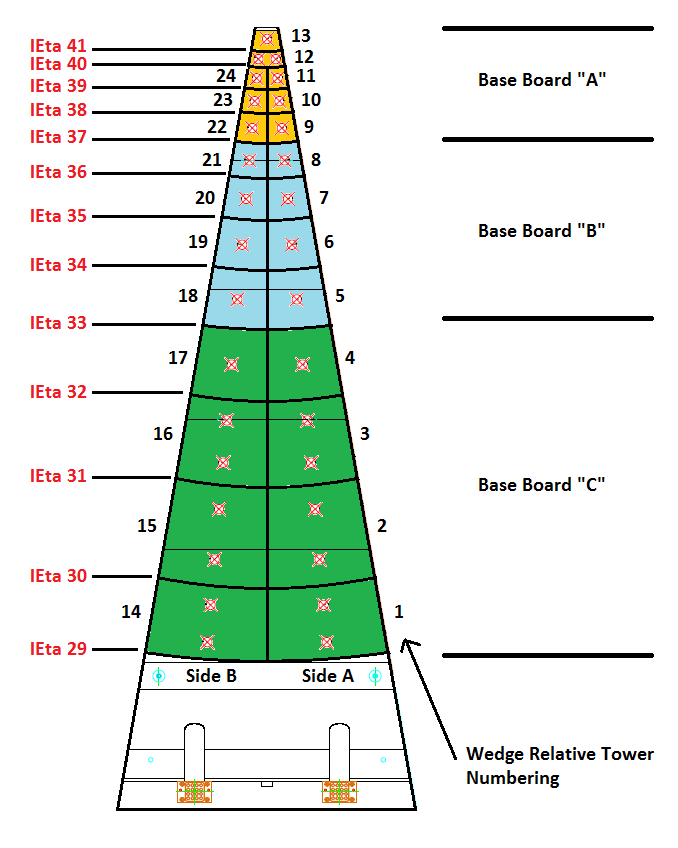
\includegraphics[width=.65\textwidth]{figures/ch_hfcalibration/HFWedge.png}
      }
      \caption{Diagram of a single HF calorimeter wedge}
      \label{fig:hf_description_wedgediagram}
   \end{center}
\end{figure}

Figure~\ref{fig:hf_description_wedgediagram} displays a transverse segmentation of a single wedge with all 24 towers and 31 source tubes. It can be seen in Figure~\ref{fig:hf_description_wedgediagram} that the geometry of each tower changes significantly between high $\eta$ index and low $\eta$ index; therefore, it is expected that the energy deposited into each tower by the passing radioactive source varies.

\begin{table}[!h] \centering \scalebox{1.10}{
  \begin{tabular}{|c|c|c|c|}
  \hline
  Tube & Mismatch & Match & Unc. \\
  \hline
  \hline
  1(14)A & 0.917 & 0.840 & 0.017 \\
  1(14)B & 0.909 & 0.833 & 0.017 \\
  2(15)A & 0.945 & 0.866 & 0.009 \\
  2(15)B & 0.938 & 0.859 & 0.009 \\
  3(16)A & 0.925 & 0.846 & 0.013 \\
  3(16)B & 0.908 & 0.829 & 0.015 \\
  4(17)  & 0.930 & 0.851 & 0.002 \\
  5(18)  & 0.889 & 0.810 & 0.003 \\
  6(19)  & 0.847 & 0.772 & 0.004 \\
  7(20)  & 0.789 & 0.713 & 0.006 \\
  8(21)  & 0.715 & 0.633 & 0.018 \\
  9(22)  & 0.646 & 0.572 & 0.006 \\
  10(23) & 0.597 & 0.516 & 0.013 \\
  11(24) & 0.498 & 0.425 & 0.023 \\
  12A(B) & 0.413 & 0.331 & 0.056 \\
  13     & 0.588 & 0.510 & 0.023 \\
  \hline
  \end{tabular}}
  \caption{Geometric correction factors for each tower's energy containment for a radioactive source
  passing through a given source tube. The value depends on what source tube contains the radioactive
  source and whether there is a match between the type of optical fiber that the source tube replaced.}
  \label{tab:hf_description_gcfactors}
\end{table}

The radioactive source excites a small region of the absorber within its immediate vicinity - 90\% of the signal output originates from a region within 3 cm of the source, with the closest optical fibers to the source contributing the most output. When performing radioactive source calibration, each tower is sourced
and analyzed separate from its neighbors; therefore, geometric correction factors must be applied to the signal output from each tower to account for the energy that escapes into neighboring towers. Monte Carlo techniques are used to account both for the energy leakage of a given tower as well as the relative position of the source tube with respect to the optical fibers (the source tubes replaced
either an EM or H type optical fiber). Table~\ref{tab:hf_description_gcfactors} lists the geometric correction factors for each tower's energy containment with respect to the type of optical fiber and the source tube replaced.

% Figure~\ref{fig:HF_Grooves} shows a matrix of groove types which identifies the  optical fiber type that was replaced by a source tube for each tower.

% \begin{figure}[!h]
%    \begin{center}
%       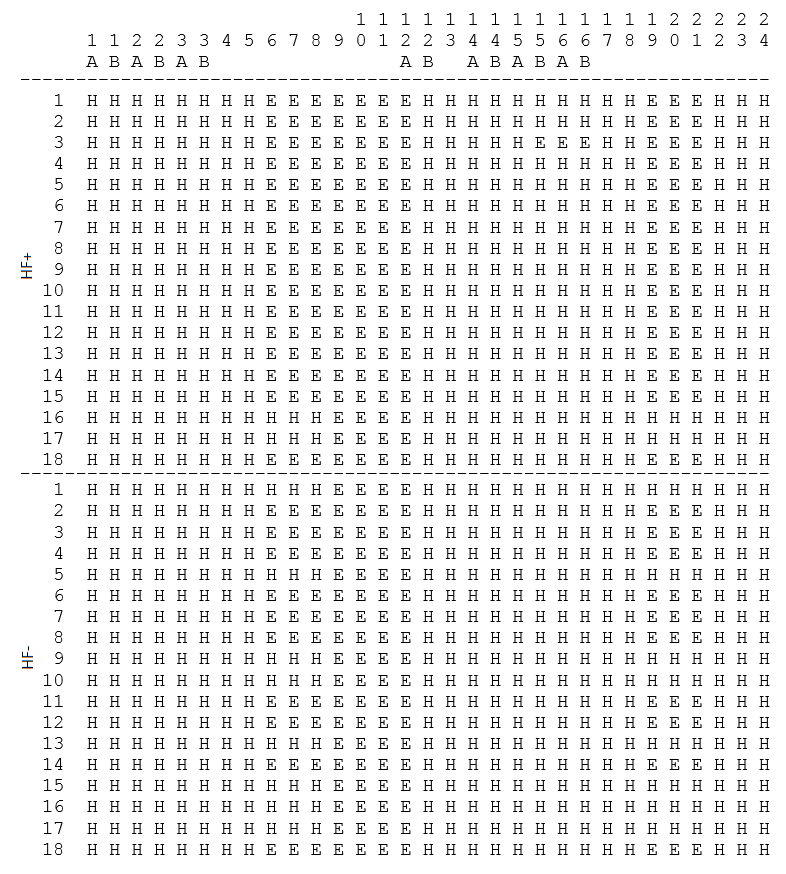
\includegraphics[width=1.\textwidth]{figures/ch_hfcalibration/Groove_Type.png}
%       \caption{Matrix of groove types that each source tube occupies within both HF
%       Calorimeters. First column is wedge number, ranging from 1-18 for each calorimeter.
%       The top row lists each source tube number for a given wedge, ranging from 1A-24.
%       Within the matrix, an E means that the source tube replaced an EM optical fiber, and
%       a H means the source tube replaced a H optical fiber.}
%       \label{fig:HF_Grooves}
%    \end{center}
% \end{figure}